\chapter{Literature Review}
\label{Chapter:Literature-Review}

As it was mentioned in Chapter \ref{Chapter:Introduction} this document proposes a system implemented on a mobile device that encourages the reduction of sedentary time via self-management techniques. In order to gain knowledge on how to devise such as system, literature review needs to be carried away on several topics. First of all, the current shift towards self-management in the health sector will be discussed. The next section will focus on evaluating how much time people spend in Sedentary Behaviour (SB) and what are the consequences. Section 3 looks at digital behaviour change techniques. Commercial and non-commercial \gls{har} mobile applications and \gls{har} itself are discussed in Section 4. Section 5 summarises the system proposed.

\section{Self-Management in the Health Sector}
 \label{section:sm-in-hs}
    Mobile devices with embedded self-management logic are currently being utilised and becoming a well-accepted solution for millions of people in the health sector. For example, the NHS’s England Executive – Simon Stevens, launched a programme “Test Beds” \citep{nhsengland2016,nhsengland2016a} which is a set of collaborative projects between NHS and some technology companies such as Verily, IBM and Philips. The idea behind the project is to test the effectiveness of different technological innovations, including wearable devices and mobile applications. These technologies will enable patients to self-manage illnesses such as diabetes, heart diseases and dementia.
    
    \subsection{Advantages of self-management}
    Shifting towards self-care via mobile devices has many advantages over the traditional methods (e.g., over the phone or face-to-face). For example, self-care devices enable patients to monitor their illnesses at home. \citet[10]{roberts2006} finds that patients using wearables improve their condition and shorten their recovery time if they can be in a familiar environment. Real-time feedback is another advantage of using self-management devices. For example, \citet{alivecor2016}, can prevent critical and even fatal incidents by identifying illness clues ahead of time. Thus, the number of patients becoming seriously ill or needing hospital treatment will potentially be reduced. Consequently, that could save money on hospital treatments \citep{campbell2016}. In addition, \citet[6]{shuger2011} found that real-time feedback on \gls{sb} could be beneficial for weight loss. \citet[97]{whitehead2016} concludes that self-management approaches delivered via mobile applications have the potential to improve outcomes of many chronic diseases.
    
    \subsection{Need for self-management devices}
    It has been found that there is a gap in the current market regarding self-care devices that focus on monitoring \gls{sb} and not only \gls{pa}. For example, \citet{sanders2016} found out that there is a lack of self-management mobile applications or devices on the market that can monitor \gls{pa}. After research, he was able to find 73 devices that provide self-monitoring of PA, and only 9 can monitor sedentary time (see Figure \ref{fig:devices-to-provide-SB-feedback}). That means that there is a lack of products in the market that offer self-management of SB in addition to PA. Sanders also concluded that the current devices capable of measuring sedentary time and providing feedback have not been used in behaviour change interventions. In conclusion, there is a need for further research and development of self-care enabled wearables to help people engage in behaviour change interventions and prevent possible chronic diseases. 
    
    \begin{figure}[h]
        \centering
        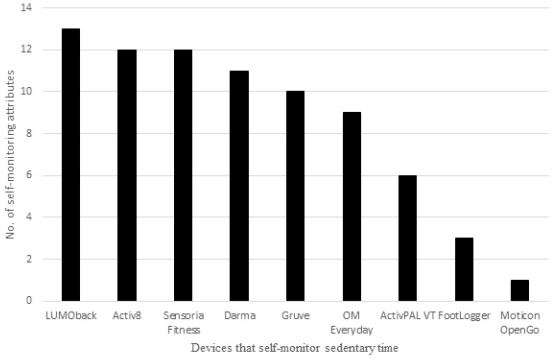
\includegraphics[width=10cm]{figureOne}
        \caption{Current technologies that self-monitor and provide feedback on SB \citep{sanders2016}}
        \label{fig:devices-to-provide-SB-feedback}
    \end{figure}

\section{Sedentary Behaviour}

Understanding the consequences of \gls{sb} as well as recommended daily energy expenditure levels is crucial for developing a mobile application that aims to implement behaviour changing theory. It is said that there is a difference between \gls{sb} and \gls{pa} and these terms should be treated differently \citep[540]{networ2012}. For example, a person can do both be sedentary for prolonged periods of time and spend large amounts of vigorous physical activity in one day. Networ define \gls{sb} as “energy expenditure less or equal to 1.5 METs while in a sitting or reclining posture” (see Table 1 for comparison of different activities). As it can be seen from Table \ref{fig:activity-intensities}, the energy spent in static activities does not result in a lot of energy expenditure and that potentially could lead to the occurrence of chronic diseases. \citet[540]{networ2012} also defines a person who is “inactive” as “not meeting specified physical activity guidelines”. That means that a person has to meet the PA recommendation levels in order to be considered as active. The next section will discuss the consequences of SB and the suggested amount of physical activity per day.

    \begin{figure}[h]
        \centering
        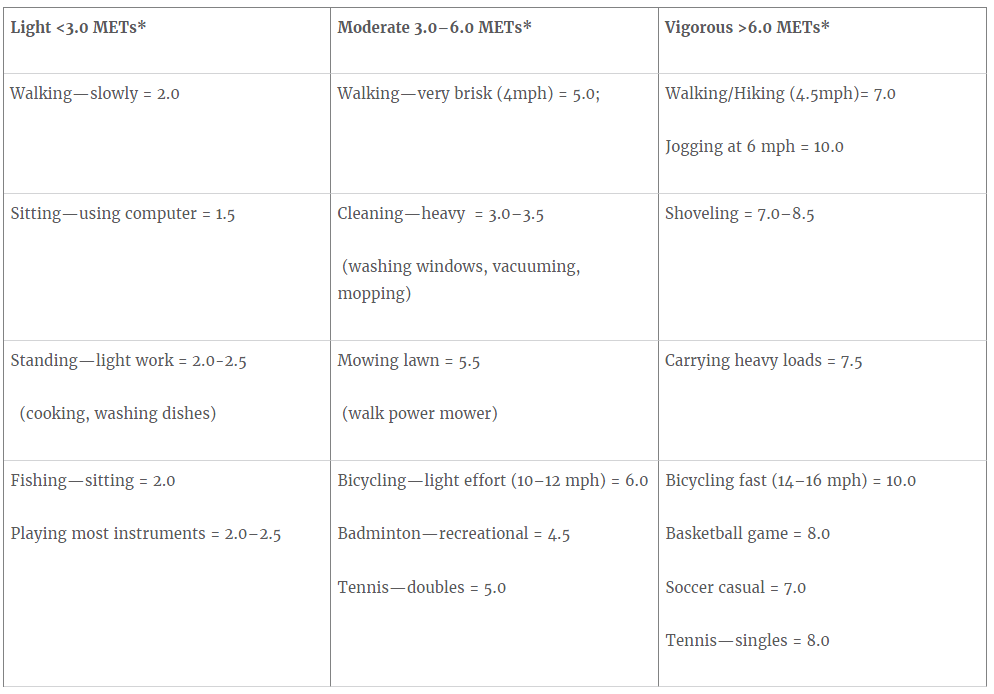
\includegraphics[width=10cm]{tableOne}
        \caption{Examples of light, moderate, and vigorous activities \citep{harvardthchanschoolofpublichealth2012}}
        \label{fig:activity-intensities}
    \end{figure}
